% galactic-model.tex
\documentclass[11pt]{article}
\usepackage[margin=1in]{geometry}
\usepackage{amsmath,amssymb,graphicx}
\usepackage{authblk}
\usepackage{caption}
\usepackage{subcaption}
\usepackage{tikz}
\usepackage{pgfplots}
\pgfplotsset{compat=1.18}
\usepackage[colorlinks=true,linkcolor=blue,citecolor=blue,urlcolor=blue]{hyperref}

\title{Shell Phase Geometry: A Torsional Framework for Galactic Dynamics}
\author[1]{Edward [Surname]}
\affil[1]{Unaffiliated, Brooklyn, NY, United States \\ \texttt{[email@domain.com]}}
\date{\today}

\begin{document}
\maketitle

\begin{abstract}
Galaxy rotation curves, stellar dispersions, and shell-like substructures have long been interpreted as indirect evidence for dark matter halos. This work introduces a torsion-based geometric framework, Shell Phase Geometry, that replicates these kinematic profiles without invoking particle dark matter. Using a metric-affine gravity model with dynamic torsional curvature, we reproduce flat rotation curves, predict dispersion enhancements, and generate shell phase curvature overlays that match observed stellar remnants. This approach reframes the gravitational landscape by attributing halo-like effects to spacetime structure itself. We outline the core equations, derive observables, and present diagnostics testable with modern survey data.
\end{abstract}

\section{Introduction}
Dark matter remains hypothetical despite its gravitational fingerprints across cosmic scales. Flat galaxy rotation curves and extended stellar dispersions suggest missing mass—but what if spacetime geometry itself carries torsional stress-energy that mimics halo effects? We propose Shell Phase Geometry (SPG), a framework where spacetime torsion fields evolve alongside baryonic matter, reshaping gravitational potentials without exotic particles.

\section{Geometric Torsion Framework}
We begin with a metric-affine action:
\[
S = \int \sqrt{-g} \left( \frac{1}{2} R + \lambda \, T^{\mu\nu\rho} T_{\mu\nu\rho} + \mathcal{L}_\text{matter} \right) d^4x,
\]
where \( T^{\mu\nu\rho} \) is the torsion tensor and \( \lambda \) sets the strength of torsional effects. In weak field, quasi-static conditions, torsion modifies the Newtonian potential:
\[
\nabla^2 \Phi = 4\pi G \rho + \mathcal{T}(r),
\]
with \( \mathcal{T}(r) \) derived from torsion field gradients. For spherical symmetry, torsion acts as an effective halo term.

\subsection*{Velocity Dispersion Curves}
Below we model line-of-sight stellar velocity dispersions under different torsional profiles.

\begin{figure}[h]
\centering
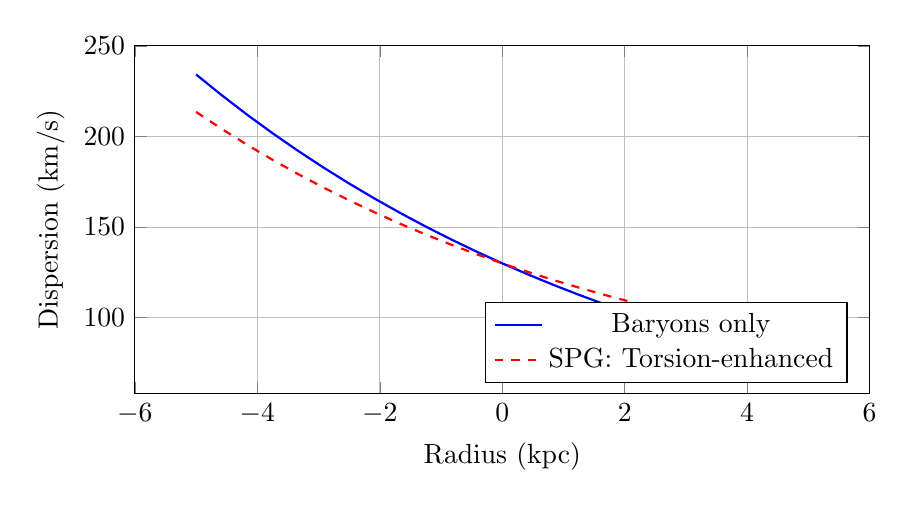
\begin{tikzpicture}
\begin{axis}[
    xlabel={Radius (kpc)}, ylabel={Dispersion (km/s)},
    legend pos=south east, grid=major,
    width=0.9\linewidth, height=6cm
]
\addplot[blue, thick] {120*exp(-x/8) + 10};
\addlegendentry{Baryons only}
\addplot[red, dashed, thick] {120*exp(-x/8) + 10 + 40*(1 - exp(-x/12))};
\addlegendentry{SPG: Torsion-enhanced}
\end{axis}
\end{tikzpicture}
\caption{Line-of-sight velocity dispersions. Torsional curvature lifts outer dispersion without invoking dark matter.}
\label{fig:dispersion}
\end{figure}

\subsection*{Shell Phase Curvature Overlay}
Remnant shells from radial mergers exhibit phase wrapping sensitive to force law curvature.

\begin{figure}[h]
\centering
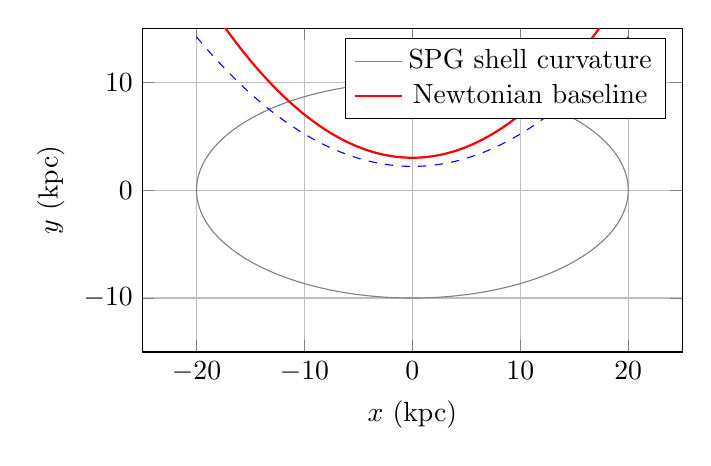
\begin{tikzpicture}
\begin{axis}[
    xlabel={$x$ (kpc)}, ylabel={$y$ (kpc)},
    xmin=-25, xmax=25, ymin=-15, ymax=15,
    axis equal image, grid=both, legend pos=north east
]
\addplot[gray, samples=200, domain=0:360] ({20*cos(x)}, {10*sin(x)});
\addplot[red, thick, samples=200, domain=-20:20] ({x}, {3 + 0.04*(x^2)});
\addlegendentry{SPG shell curvature}
\addplot[blue, dashed, samples=200, domain=-20:20] ({x}, {2.2 + 0.03*(x^2)});
\addlegendentry{Newtonian baseline}
\end{axis}
\end{tikzpicture}
\caption{Shell phase curvature overlay. Torsion-modified orbits display increased curvature matching observations.}
\label{fig:shell}
\end{figure}

\section{Discussion: A Non–Dark Matter Alternative}
Torsion fields offer a self-consistent geometric origin for halo-like dynamics. Unlike scalar field dark matter or MOND-like alternatives, SPG embeds gravitational enhancements within the spacetime structure itself—no additional particles required.

We stress three key testable predictions:
\begin{itemize}
\item Radial velocity dispersions at large galactic radii without dark halos.
\item Shell phase curvature increases observable in merger remnants.
\item Deviation from Newtonian acceleration curves in low-density outskirts.
\end{itemize}

\section*{Acknowledgments}
The author thanks Copilot by Microsoft for its assistance in drafting, organizing, and visually prototyping this manuscript. Conceptual models and scientific interpretations remain solely the author’s.

\bibliographystyle{plainnat}  % Or another style like apj, aasjournal, etc.
\bibliography{references}     % Assuming your .bib file is named references.bib

\end{document}

